 
\documentclass[12pt]{article}
%authors Andrew Schneider, David Dobor
\usepackage[margin=1in]{geometry} 
\usepackage{amsmath,amsthm,amssymb}
 \usepackage{graphicx}
 \usepackage{multirow}
\usepackage[scaled]{helvet}
\usepackage{hyperref}
\usepackage[usenames,dvipsnames,svgnames,table]{xcolor}
\usepackage[T1]{fontenc}
\usepackage{palatino}
\usepackage{enumerate}
%\renewcommand*\familydefault{\sfdefault} %% Only if the base font of the document is to be sans serif

\newcommand{\N}{\mathbb{N}}
\newcommand{\Z}{\mathbb{Z}}


\newcommand{\blditA}{\textbf{\textit{A}}}
\newcommand{\blditB}{\textbf{\textit{B}}}
\newcommand{\blditC}{\textbf{\textit{C}}}
\newcommand{\blditP}{\textbf{\textit{P}}}
\newcommand{\blditQ}{\textbf{\textit{Q}}}
\newcommand{\bldI}{\textbf{I}}
\newcommand{\blditX}{\textbf{\textit{X}}}
\newcommand{\blditY}{\textbf{\textit{Y}}}
\newcommand{\blditZ}{\textbf{\textit{Z}}}
 
\newenvironment{theorem}[2][Theorem]{\begin{trivlist}
\item[\hskip \labelsep {\bfseries #1}\hskip \labelsep {\bfseries #2.}]}{\end{trivlist}}
\newenvironment{lemma}[2][Lemma]{\begin{trivlist}
\item[\hskip \labelsep {\bfseries #1}\hskip \labelsep {\bfseries #2.}]}{\end{trivlist}}
\newenvironment{exercise}[2][Exercise]{\begin{trivlist}
\item[\hskip \labelsep {\bfseries #1}\hskip \labelsep {\bfseries #2.}]}{\end{trivlist}}
\newenvironment{problem}[2][Problem]{\begin{trivlist}
\item[\hskip \labelsep {\bfseries #1}\hskip \labelsep {\bfseries #2.}]}{\end{trivlist}}
\newenvironment{question}[2][Question]{\begin{trivlist}
\item[\hskip \labelsep {\bfseries #1}\hskip \labelsep {\bfseries #2.}]}{\end{trivlist}}
\newenvironment{answer}[2][Answer]{\begin{trivlist}
\item[\hskip \labelsep {\bfseries #1}\hskip \labelsep {\bfseries #2.}]}{\end{trivlist}}

\begin{document}
 \renewcommand{\arraystretch}{1.3}

 
\title{Stat 8003, Homework 5}%replace X with the appropriate number
\author{Group G: \ \ \texttt{sample( c( "David" , "Andrew",  "Salam" ))}
\\ %replace with your name
} %if necessary, replace with your course title
 
\maketitle
 
 %%%%%%%% Question 1 %%%%%%%%%
 \begin{question}{5.1}  
 
 Consider a simulated dataset. Assume that the data $x_1, x_2, \cdots , x_n$ follows the following distribution:
 $$
 x_i \sim f(x_i) = \pi_0 f_0(x_i) + \pi_1 f_1(x_i)
 $$
 where $f_0(x_i) = 1(0 \leq x_i \leq 1)$ is the density function of the uniform and $f_1(x_i) = \beta (1 - x)^{\beta - 1} $ is the density function of $Beta(1, \beta)$. The group information can be treated as a
missing value and is denoted as $z_i$. Let $y_i = (x_i, z_i)$ be the complete data.	
 \begin{enumerate}[(a)]
\item Derive the complete likelihood function;
\item Use the EM algorithm to derive the estimator for $\pi_0$ and $\beta$;
\item Apply your method to the data set, estimate $\pi_0$ and $\beta$ and the calculate $\text{\texttt{fdr}}_i = P(Z_i = 0 \mid x_i)$. (This score is called the local \texttt{fdr} score.)
\item Classify $x_i$ to the first group if $\text{\texttt{fdr}}_i(x_i) > 0.5$. Compare your classification with the actual
group information, what is the total number of falsely classified data?
\end{enumerate}
\end{question} 


  \textbf{\color{TealBlue}\emph{Answer:} } 
    
  
\begin{enumerate}[(a)]  
\item First, the \emph{incomplete} likelihood function is given to be:
  $$
  L(\theta \ ; \blditX) = \prod_{i=1}^n \left(   \pi_0 1 + \pi_1 \beta (1 - x_i)^{\beta - 1}   \right)
  $$



Then the \emph{complete} likelihood function is:
$$\boxed{
L(\theta \ ; \blditY) = \prod_{i=1}^n \left( 1 (Z_i = 0) \ \pi_0  + 1( Z_i = 1) \ \pi_1 \ \beta (1 - x_i)^{\beta - 1} \right) }
$$ 
  
  An alternative way of writing this likelihood is:
  \begin{align*}
   f(x_i, z_i \mid \theta) = 
  \begin{cases}
  \pi_0 \; \; \; \; \; \; \; \; \; \; \; \; \; \; \; \; \; \; \; \; \; \; \; \; \; \text{if} \; Z_i = 0\\
  \pi_1 \ \beta (1 - x_i)^{\beta - 1}\; \; \; \; \; \text{if}  \; Z_i = 1\\
  \end{cases}
  \end{align*}


%%%%% part b) the Q function and parameter estimates
\item To get the estimates for $\pi_0$ and $\beta$, we first find the expected value of the \emph{log} of the \emph{complete likelihood} function with respect to $Z$ (the so called $Q$ function). As in the notation used in class, let $\theta^t$ stand for the parameter estimates obtained at iteration $t$ of the EM algorithm (so $\theta^t = (\pi_0^t, \beta^t)$).

\begin{align*}
Q(\theta \mid \theta^t) &= \mathrm{E} \; \log (L(\theta \ ; \blditY) ) \\
&= \mathrm{E} \; \log \left( \prod_{i=1}^n \left( 1 (Z_i = 0)\ \pi_0   + 1( Z_i = 1)\ \pi_1  \ \beta (1 - x_i)^{\beta - 1} \right) \right)\\
&= \mathrm{E} \; \left[ \sum_{i=1}^n  \log \left( 1 (Z_i = 0)\ \pi_0   + 1( Z_i = 1)\ \pi_1 \ \beta (1 - x_i)^{\beta - 1} \right) \right] \\
\end{align*}
  
  The last expression in the brackets is either $\log(\pi_0)$ or $ \log(\pi_1\ \beta (1 - x_i)^{\beta - 1})$, depending on the outcome of $Z$. So
  
\begin{align*}
Q(\theta \mid \theta^t) &= \sum_{i=1}^n \left( \; \; \mathrm{E} \; 1 (Z_i = 0)\ \log(\pi_0) + \mathrm{E} \; 1 (Z_i = 1)\ \log(\pi_1\ \beta (1 - x_i)^{\beta - 1}) \; \; \right) \\
&= \sum_{i=1}^n \left( \; \; P(Z_i = 0 \mid x_i, \theta)\ \log(\pi_0) +  P(Z_i = 1 \mid x_i, \theta)\ \log(\pi_1\ \beta (1 - x_i)^{\beta - 1}) \; \; \right) \\
\end{align*}
  
  Where the last equality follows because the expectation of the indicator function of a \texttt{r.v.} is simply the probability of the corresponding event. \\
  \\
  These probabilities will be computed using Bayes rule and denoted by $T_{ij}^t$:
\begin{align*}  
T_{ij}^t &= P(Z_i = j \mid x_i, \theta) = \frac{P( x_i \mid Z_i = j) P(Z_i = j) } {\sum_{j=0}^1  P( x_i \mid Z_i = j) P(Z_i = j) }  \; \; \; \; \text{for} \; \; j = 0, 1 \\
\end{align*} 
Thus
$$
T_{i0}^t = \frac{\pi_0^t}{\pi_0^t + \pi_1^t \ \beta^t (1 - x_i)^{\beta^t - 1}} 
$$
\\
$$
T_{i1}^t = \frac{\pi_1^t \ \beta^t (1 - x_i)^{\beta^t - 1}} { \pi_0^t + \pi_1^t \ \beta (1 - x_i)^{\beta^t - 1} }
$$
(where the superscript $^t$ marks the values of the parameters obtained at the the $t$-th iteration.)

Rewriting the $Q$ function:
\begin{align*}
Q(\theta \mid \theta^t) &= \sum_{i=1}^n \left( \;  T_{i0}^t \log(\pi_0) + T_{i1}^t \log(\pi_1\ \beta (1 - x_i)^{\beta - 1}) \; \right) \\
&= \sum_{i=1}^n \left(\;  T_{i0}^t \log(\pi_0) + T_{i1}^t \log(1 - \pi_0) \ + T_{i1}^t \log (\beta (1 - x_i)^{\beta - 1} \;  \right) \\
\end{align*}

We maximize it with respect to $\pi_0$ and $\beta$. Setting $Q$'s partial derivatives to zero,
\begin{align*}
\frac{d}{d\pi_0} Q(\theta \mid \theta^t) &= \sum_{i=1}^n \left( \; \; 
 T_{i0}^t \frac{1}{\pi_0} - T_{i1}^t  \frac{1}{1 - \pi_0} \; \; \right) = 0\\
%\end{align*}
%\begin{align*}
\frac{d}{d\beta} Q(\theta \mid \theta^t) &= \sum_{i=1}^n \left( \; \; 
T_{i1}^t  \frac{1}{\beta} + T_{i1}^t \log(1 - x_i)\; \; \right) = 0\\
\end{align*}
We obtain
$$\boxed{
\pi_0^{t+1} = \frac{\sum_{i=1}^n T_{i0}^t } {\sum_{i=1}^n \left( T_{i0}^t + T_{i1}^t \right)} = \frac{\sum_{i=1}^n T_{i0}^t } {n} }
$$
$$\boxed{
\beta^{t+1} = \frac{-\sum_{i=1}^n T_{i1}^t  } {\sum_{i=1}^n T_{i1}^t \log(1 - x_i) } }
$$
\\

%%%%% part c)  use the data set to obtain concrete estimates for parameters
\item
The EM algorithm converges to the following values of $\theta$ (code attached separately):
$$\boxed{
\pi_0 = 0.696794 \; \; \; \text{and} \; \; \; \beta = 11.093249 }
$$
We use these parameters to obtain the \texttt{fdr} score for the $i^{\text{th}}$ observation as follows:
$$
\text{\texttt{fdr}}_i  = P(Z_i = 0 \mid x_i) =  T_{i0} = \frac{\pi_0}{\pi_0 + \pi_1 \ \beta (1 - x_i)^{\beta - 1}}
$$

The following code snippet was used to obtain the \texttt{fdr} scores:
\begin{verbatim}
# X.value # this is the given data
# beta # = 11.093249 , obtained by running EM algorithm
# pi0 # 0.696794 , obtained by running EM algorithm

fdr_score <- pi0 / (pi0 + pi1*beta*(1 - X.value)^(beta - 1))  


\end{verbatim}

%%%%% part d)  classify data according to fdr score
\item
We can now classify data using the criterion that a data point belongs to the first group if its \texttt{fdr} score exceeds $0.5$ and that it belongs to the second group otherwise. We can then compare our classification result with the actual group information:

\begin{verbatim}
##Find the local fdr and compare it with the data

greater_than_half = function(x){
    if( x > 0.5)
        0
    else
        1
}

fdr_score <- pi0 / (pi0 + pi1*beta*(1 - X.value)^(beta - 1))
Z.guess <- sapply(fdr_score,greater_than_half)

falsely_classed <- sum(abs(Z.guess - X.group))   # =321
\end{verbatim}

Thus only 321 out of 2000 got falsely classified (about 16\%). 

\end{enumerate}

\vspace{1000 mm}

%\begin{verbatim}
%\end{verbatim}

\bigskip
\bigskip
 %%%%%%%% Question 2 %%%%%%%%%
 \begin{question}{5.2} (Continued from Problem 1.)  It is known that the local fdr score can be written as 
$$
fdr_i(x_i) = \frac{\pi_0 f_0(x_i)} {f(x_i)}
$$
where $f(x_i)$ is the marginal density of $x_i$. Assume that $\pi = 0.7$.
 \begin{enumerate}[(a)]
\item Estimate $f(x_i)$ by using the kernel density estimation with Gaussian kernel and Silverman's $h$;
\item Estimate the local \texttt{fdr} score;
\item  Using the same rule as in 1(d), calculate the total number of falsely classified data;
\item Choose the bandwidth using the maximum likelihood cross validation, repeat problem (a-c),
what is the total number of falsely classified data?
\item Which method works the best in terms of having the smallest classification error?
\end{enumerate}
\end{question} 


  \textbf{\color{TealBlue}\emph{Answer:} } 
 
\begin{enumerate}[(a)]
\item Using the Gaussian kernel, and Silverman's $h$, our density estimate looks like this:

\begin{center}
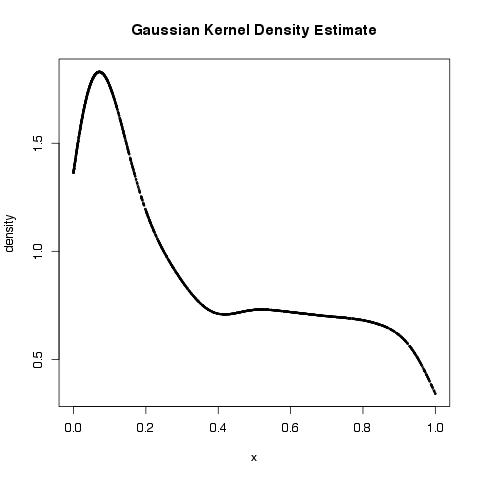
\includegraphics[width=10cm, height=10cm]{plot_prob2_a}
\end{center} 
(The code that generates this figure is submitted separately.)

\item From part (a) we are able to estimate density at each observation $x_i$. We use the following formula to compute the \texttt{fdr} score:
\\
$$
\text{\texttt{fdr}}_i = \frac{0.7} {\text{value of the estimated density } f(x_i)}
$$
\\
The following code snippet does this computation in \texttt{R}:
\begin{verbatim}
pi0 <- 0.7
n <- length( X.value )
h <- 1.06 * sqrt( var(X.value) ) / (n^(1/5))

k_estimate = function(x){
    1/(h) * mean( dnorm( (x - X.value)/h, 0, h))
}

X.kdestimate <- pi0 / sapply(X.value,k_estimate)
\end{verbatim}

\item The total number of falsely classified observations using the score turns out to be 318:
\begin{verbatim}
X.kdestimate <- pi0 / sapply(X.value,k_estimate)
Z.guess.kde <- sapply(X.kdestimate,greater_than_half)

falsely_classed2 <- sum(abs(Z.guess.kde - X.group)) #answer: 318
\end{verbatim}

\item We now choose a different bandwidth $h$ using the \texttt{kedd} library. Here $h$ turns out to be higher than Silverman's $h$: $\text{\texttt{h.cv}} = 0.1058126$.
\begin{verbatim}
library(kedd)
h <- h.mlcv(X.value)$h    # output: h.cv = 0.1058126
\end{verbatim}

Repeating steps (a) - (c) with this new $h$ gives:
\begin{verbatim}

X.kdestimate.cv <- pi0 / sapply(X.value,k_estimate)
Z.guess.kde.cv <- sapply(X.kdestimate.cv,greater_than_half)

falsely_classed3 <- sum(abs(Z.guess.kde.cv - X.group)) # answer: 325
\end{verbatim}

With the new bandwidth, we get a slightly higher number of falsely classified data. 

The number of falsely classified here is 325.


\item Which method works best? We expected cross-validation to work better, but it actually gave worse results: 325 falsely classified as opposed to 318 falsely classified with Silverman's h. The difference isn't great, but among the three estimates used here, Silverman's h gave us the lowest number of falsely classified.
 \end{enumerate}

\end{document}

%Rewriting the $Q$ function:
%\begin{align*}
%Q(\theta \mid \theta^t) &= \sum_{i=1}^n \left( \frac{\pi_0 \ \log(\pi_0) \ + \ \pi_1 \ \beta (1 - x_i)^{\beta - 1} \log(\pi_1\ \beta (1 - x_i)^{\beta - 1})} {\pi_0 + \pi_1 \ \beta (1 - x_i)^{\beta - 1}} \right) \\
%&= \sum_{i=1}^n \left( \frac{\pi_0 \ \log(\pi_0) \ + \ \pi_1 \ \beta (1 - x_i)^{\beta - 1} \log(\pi_1\ \beta (1 - x_i)^{\beta - 1})} {\pi_0 + \pi_1 \ \beta (1 - x_i)^{\beta - 1}} \right) \\
%\end{align*}
%
%We can express this in terms of $\pi_0$ and $\beta$ only:
%\begin{align*}
%Q(\theta \mid \theta^t) &= \sum_{i=1}^n \left( \frac{\pi_0 \ \log(\pi_0) \ + \ (1 - \pi_0) \ \beta (1 - x_i)^{\beta - 1} \log((1 - \pi_0)\ \beta (1 - x_i)^{\beta - 1})} {\pi_0 + (1 - \pi_0) \ \beta (1 - x_i)^{\beta - 1}} \right) \\
%&= \sum_{i=1}^n \left( \frac{\pi_0 \ \log(\pi_0) \ + \ (1 - \pi_0) \ \beta (1 - x_i)^{\beta - 1} ( \log((1 - \pi_0)\ + \log (\beta (1 - x_i)^{\beta - 1}) )} {\pi_0 +  \ \beta (1 - x_i)^{\beta - 1} - \pi_0 \beta (1 - x_i)^{\beta - 1} }\right) \\
%\end{align*}
%\begin{align*}
%\sum_{i=1}^n \left( \frac{\pi_0 \ \log(\pi_0) \ + \ (1 - \pi_0) \ \beta (1 - x_i)^{\beta - 1} \log((1 - \pi_0)\ + \ (1 - \pi_0) \ \beta (1 - x_i)^{\beta - 1} \log (\beta (1 - x_i)^{\beta - 1}) )} {\pi_0 +  \ \beta (1 - x_i)^{\beta - 1} - \pi_0 \beta (1 - x_i)^{\beta - 1} }\right) 
%\end{align*}
%
